\section{Descripción del código del proyecto.}

\subsection{Composición del proyecto.}
En esta sección se hará una descripción de cómo está compuesto el proyecto, indicando el uso de 
carpetas y el contenido en cada una de estas.
\\\\
En este proyecto se muestran 3 carpetas que permiten la separación del código en partes lógicas que
permite el funcionamiento del proyecto.

%\begin{wrapfigure}{l}{0.25\textwidth}
%    \centering
%    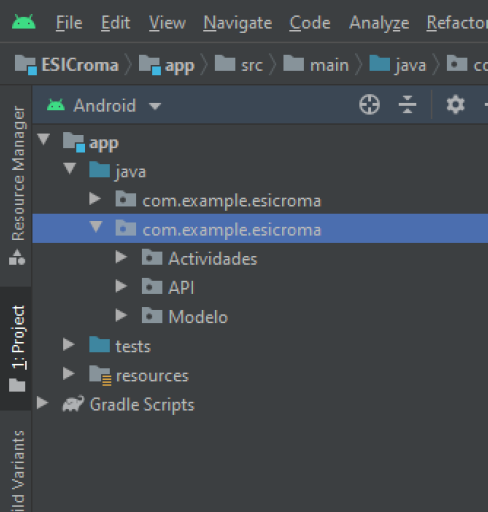
\includegraphics[scale=0.5]{Imagen/Android.png}
%{contour}
%\end{wrapfigure}

% paragraph
\begin{multicols}{2}
    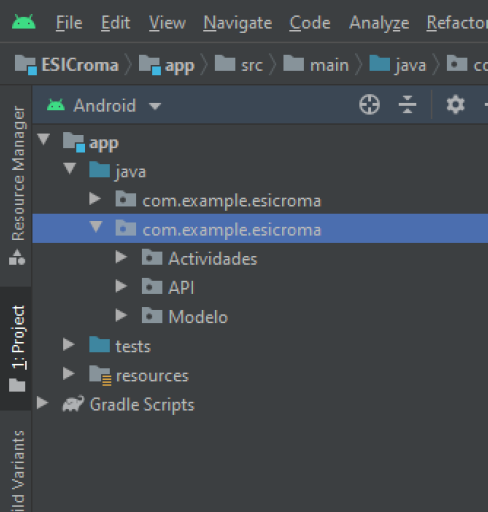
\includegraphics[width=0.43\textwidth]{Imagen/Android.png}
    
    \begin{itemize}
        \item Carpeta Actividades: En esta carpeta se almacenan todas las clases de la lógica para el 
        funcionamiento de las Actividades (Parte lógica de lo visual).
        \item Carpeta API: Esta carpeta almacena las clases lógicas que permiten la comunicación del 
        Back-End y la aplicación.
        \item Carpeta Modelo: En esta carpeta almacena el modelado de las peticiones que se piden al Back-End
    \end{itemize}
\end{multicols}


\subsection{Carpeta Actividades.}
Se procede a explicar los componentes de cada clase que almacena esta carpeta.

\subsubsection{Clase A\_IniciarSesion.}
En esta clase se hacen los procesos que permite hacer el inicio de sesión con las siguientes funciones:

\paragraph {EnableRuntimePermissionToAccessCamera:} Esta función permite que la aplicación al momento de abrirla, 
muestre una ventana pidiendo el permiso del uso de la cámara.

\paragraph {Validar\_Email:} Esta función recibe un parámetro de tipo String y permite validar si el texto proporcionado 
en el campo donde se ingresa el correo, evalúa si es un correo electrónico bien escrito.

\paragraph {Ir\_A\_La\_Pantalla\_de\_Perfil:} Esta función permite que la aplicación cambie de ventana, y pueda abrir la ventana de perfil.

\paragraph {Iniciar\_Sesion:} Esta función permite almacenar la información de los campos de texto (correo y contraseña) en variables 
con los mismos nombres, el cual hace una petición al back-end enviando la información almacenada en las dos variables y recibiendo 
la respuesta que el back-end envía, esta función evalúa la respuesta del back-end y en caso de que la información recibida no sea 
válida permanece en la misma ventana, en caso contrario esta función hace que guarde la respuesta del back-end en una variable con 
el nombre de Datos\_De\_Usuario y cambia de ventana usando la función Ir\_A\_La\_Pantalla\_de\_Perfil.


\subsubsection{Clase B\_Perfil.}
En esta clase solo se encuentran 2 funciones que permiten cambiar de ventana.

\paragraph {Ir A\_La\_Pantalla\_De\_Crear\_Muestra:} Esta función permite cambiar de ventana y muestra la ventana de C\_Crear\_Muestra.

\paragraph {Ir A\_La\_Pantalla\_De\_Guardar\_Localizacion:} Esta función permite cambiar de ventana y muestra la ventana de E Guardar Coordenadas.

\subsubsection{Clase C\_Crear\_Muestra.}
En esta clase es donde se hace el análisis de la muestra, hace una petición y recibe la respuesta del back-end.

\paragraph {Ir\_A\_La\_Pantalla\_De\_Resultados:} Esta función permite cambiar de ventana y muestra la ventana de Pantalla De Resultados.
    
\paragraph {takePictureIntent:} Esta función permite tomar la fotografía.
    
\paragraph {postFile:} Esta función permite enviar la fotografía tomada y recibir respuesta del servidor con el análisis hecho, esta misma 
función permite cambiar de ventana cuando recibe la respuesta del servidor y se dirige a la ventada D Analisis Croma.

\paragraph {Lista\_De\_Lugares:} Esta función permite traer la información de los lotes del usuario que ha iniciado sesión.

\paragraph {Datos\_Region:} Esta función permite traer los datos de municipio, estado y país del usuario que ha iniciado la sesión.
    
\paragraph {Informacion\_Muestra:} Esta función recibe un parámetro de tipo int es el identificador del croma, esto para hacer una petición 
al back-end y como respuesta del back-end se reciba los datos de la muestra.
    
\paragraph {Datos\_de\_la\_Muestra:} Esta función recibe un parámetro de tipo int que es el identificador del croma, esta petición al back-end 
y recibe como respuesta la información de todo el croma, la misma función muestra la latitud y longitud de la muestra tomada y se muestra 
para que el usuario sepa cuales son las coordenadas donde se tomó su muestra.
    
\paragraph {FormatoDecimal:} Esta función recibe un parámetro de tipo String y permite reducir la cantidad de decimales de un número.
    
\paragraph {displayUserData:} Esta función recibe un parámetro de tipo Object esta variable almacena toda la información del lote del 
usuario y esta función permite colocar en la parte visual el nombre del lote.

\subsubsection{Clase D\_Analisis\_Croma.}
En esta clase solo se hace uso de 3 de funciones para registrar los datos del croma analizado en la base de datos.

\paragraph {Cambio\_de\_Colores:} Esta función se utiliza para hacer cambio de colores en la parte visual de los campos donde se detectan 
que hay existencia de los componentes busados en el croma.
    
\paragraph {Actu\_CRM:} Esta función permite traer la información de un croma, para eso necesita 2 parámetros los cuales son uno de tipo int 
y otro de tipo Object, que con eso la función hace una petición al back-end.
    
\paragraph {subir\_Imagen:} Esta función permite almacenar la fotografía que se tomó, al servidor.

\subsubsection{Clase E\_Guardar\_Coordenadas.}
Esta clase permite obtener y guardar las coordenadas de la ubicación de donde la muestra que se obtuvo.

\paragraph {Permiso\_De\_Localizacion:}
    Esta función permite que muestre una ventana pidiendo el permiso del uso de la localización (GPS).
    
\paragraph {Obtener\_Coordenadas:} Esta función permite obtener las coordenadas, almacena la información 
en 2 variables (latitud y longitud) y las muestra en los campos respectivos en la parte visual del proyecto.

\paragraph {nuevo\_lista:} Esta función hace una petición al back-end para traer información de los lotes, el 
cual se muestran de forma visual los nombres de cada lote registrado por el usuario.

\paragraph {lista\_de\_medidas:} Esta función muestra de forma visual la lista de medidas que se toman para extraer 
la muestra de cada croma.

\paragraph  {Guardar\_Informacion:} Esta función permite guardar el nombre de la muestra que se tomó y también permite 
guardar las coordenadas de donde se obtuvo la muestra a la base de datos.

\subsection{Carpeta de API.}
Se procede a explicar los componentes de cada clase que almacena esta carpeta.

\subsubsection{Clase API.}
En esta clase se hace todas las peticiones que se solicitan al servidor, para obtener respuesta de lo solicitado.

\subsubsection{Clase ClienteRetrifit.}
Esta clase está orientada a la conexión con los servidores y tener respuestas con el back-end.

\paragraph {ClienteRetrofit:} Esta función permite conectarse al servidor donde se aloja el back-end de la información 
de usuario, etc.
    
\paragraph {ClienteRetrofit con parámetro:} Esta función recibe un parámetro de tipo String el cual tiene como propósito 
conectarse con el servidor que aloja el servicio de análisis del croma.

\paragraph {getInstance:} Esta función permite crear una instancia de la conexión del CLienteRetrofit.
    
\paragraph {getInstance2:} Esta función permite crear una instancia de la conexión del CLienteRetrofit con parámetro.
    
\paragraph {getApi:} Esta función retorna la conexión hecha.


\subsection{Carpeta de Modelo.}
En esta carpeta se almacenan todas las clases con el modelo que pertenecen respecto a las respuestas que el back-end envía a través de JSON.